\documentclass[12pt,a4]{article}
% \raggedright
% \parindent0pt \parskip8pt
\usepackage{hyperref}
\usepackage{url}

\usepackage{graphicx}
\usepackage{wrapfig}
\hypersetup{
  pdftitle = {Semantic Web Search},
  pdfauthor = {Milan Thapa},
  pdfsubject = {AI Research Paper},
  pdfkeywords = {Sementic Web, Reveiw Paper, Latex},
  colorlinks=true,
  linkcolor=black,
  urlcolor=blue,
  citecolor=black,
}

\title{Report On Semantic Web Search}
\author{Milan Thapa(52)}
\date{\today}
%document begins from here...:)
\begin{document}
%imported cover page from a tex file...:D
\pagenumbering{none}
\thispagestyle{empty}

\makeatletter
\setlength\@fptop{0pt}
\setlength\@fpsep{20pt plus 2pt minus 2pt}
\setlength\@fpbot{0pt}
\makeatother

\begin{table}[t]
  \begin{tabular}{c}
   % \begin{center} 
      \Huge{\bf{Semantic Web Search}} \\\\
      \large{\textit{\bf Review Paper}}\\\\
      \today\\\\\\
      
%\begin{wrapfigure}{t}{8em}
      
\includegraphics[height=6cm]{./img/ku_logo.png}\\\\\\
      % \end{wrapfigure}

      \large{Submitted to}\\\\
      \Large{\bf Mr. Santosh Khanal}\\\\\\
      \large{\bf Deptartment of Computer Science and Engineering}\\\\
      \large{\bf Kathmandu University}\\\\
      \large{\bf Dhulikhel, 5 Kavre}\\\\ \\\\      

      \large{Submitted by} \\\\
      \Large{\bf Milan Thapa (52)}\\
      \large{Semester 7}\\
      \large {\href{mailto:milans.thapa78@gmail.com}{milans.thapa78@gmail.com}}
      

   % \end{center}
\end{tabular}  
\end{table}

\clearpage
\pagenumbering{roman}
\setcounter{page}{2}
\tableofcontents
\newpage
\section{Introduction}
% \rule{\textwidth}{0.5pt}
\pagenumbering{arabic}
\subsection{Search History before Semantic Web}
From the invention of the internet and web, the inforamtions and data are being accumulated, refined and distributed all over the world. Up to par, the web have been through its different versions. \textbf{Web 1.0} was all about the \textit{information web}, where people just collected the data over the network. It got advanced to \textbf{Web 2.0} as a \textit{social web} when people started getting connectd through social networking like hi5,linkdien,facebook. Meanwhile the data accumulation rate over the web got its exponential hit and the process is still being growing progressively. The search engines during the days of web 2.0  were just programmed to serve the user's query with some algorithms of page ranking \textit{like Goolge PageRank in old days to predicate relevant result, before its knowledge graph}. With those chaos of the information all over the web, a user using some searching techniques like: the user provided a phrase which is intended to denote an object of which the user was trying to gather information about. But the poor search engines couldn't exactly resolve the phrase user was actually looking for, it is because the engines really didn't have any idea(clue) of what informations and data they were dealing with. They were just programmed, without any intillegence to analyse the meaning of a simple phrase. So with no altenatives, the user tried to locate a number of documents or pages which together would give him/her the information s/he was really after.\begin{quote}\textit{i.e. every time a user needed a information about something, s/he became an explore, exploring the web, filtering the contents, merging all together and finally drawing some desired meaning out of those.--- number of procedures to do simple search.}\end{quote}
So that is why \textbf{semantic web} emerged as an extension of the current web by standards and technologies that help machines to understand the information on the Web, to support richer discovery, data integration, navigation, and automation of tasks.
\clearpage
\subsection{Semantic Web ---an Intelligent Web}
Semantic web ---an intillegent web is a web designed to solve all the chaos of informations and data spreading all over the current internet. It's an evolving collection of knowledge, built to allow anyone on the Internet to add what they know and find answers to what they want to know\cite{Sandro} Information on the Semantic web, rather than being in natural language text, is maintained in a structured form which is fairly easy for both computers and people to interact and work with. 
% \begin{comment}What is semantic web search\end{comment}
The mechanism of linking the search engine to the semantic web give rise to the new terminology called semantic web search or so called semantic search. Its a search engine designed to improve search accuracy by understanding searchers intent and the contextual meaning of terms as they appear in the searchable dataspace (on the web), to generate more relevant results. As an explanatory example
\begin{quote}\textit{When searching for ''laptop'', then one is looking for laptops or synonyms / related concepts (such as ''notebook''), but also for special kinds of laptops that are not synonyms / related concepts, such as e.g. IBM/Lenovo ThinkPads. That is where web needs an intelligence and reply the desired results.ie semantic search.}\end{quote}

One important goal of the semantic web is to make the meaning of information explicit through semantic mark-up, thus enabling more effective access to knowledge contained in heterogeneous information environments, such as the web. Semantic search plays an important role in realizing this goal, as it promises to produce precise answers to user’s queries by taking advantage of the availability of explicit semantics of information. Another example could be like this: when searching for news stories about ''UNG students'', with traditional searching technologies, we often could only get news entries in which the term ''UNG students" appears. Those entries which mention the names of students but do not use the term ''UNG students" directly will be missed out. Such news entries however are often the ones that the user is really interested in. In the context of the semantic web, where the meaning of web content is made explicit, the semantic meaning of the keyword (which is a general concept in this example of UNG students) can be figured out. Furthermore, the underlying semantic relations of metadata can be exploited to support the retrieving of information which is closely related to the keyword. Thereby, the search performance can be significantly improved by expanding the query with instances and relations.

\subsection{Why Semantic Web Search ?}
The effective exploration of the web content involves with the numerious challanges like:
\begin{description}
\item[Useability] The user on a web searching for something does't care how the structured query is specified. The end user often does not know the query language and the underlying data scheme. For example searching pdf,docs,tex in google one simply couldnot know that use of tag filetype:pdf/doc/tex could be handy.
\item[Scalability] As the amount of available data is ever growing, the ability to scale the most desired results is essential.
\item[Imprecise Information Needs] The information needs expressed by the user might be imprecise. An effective search solution should be able to consider this aspect to deliver relevant results. For example: a user might search phrases like vdo for video,fbk for facebook,anime for animation,b4 for before, bday for birthday, etc. 
\item[Data Change] The Web of Data is continuously changing. Thus, efficient mechanisms for index update at the Web scale are needed when data changes. 
\end{description}
So understanding the user's intent by analysing keywords he/she is trying to search with the aid of dynamic web resources knowledge scattered over the internet is the first thing what semantic search is designed for. Thus it explored the possibility of search engines with a broad sense that a user happily could trust the search results that matched his/her intention. He/she can always put search phrase in clean and simple search interface with zero knowledge of any syntax and procedures, i.e, in his/her own ways and with his/her own language.


The need of the semantic search or semantic web is fundamental aspect of the current web.It could be generalise with some simple examples:
\begin{description}
\clearpage
\item[Example1:] From the interview of Sir Tim Berns Lee \textit{''Looks Back The InWeb Addresses Was Unnecessary\cite{tim}''} ,he had had and exmaple of going to an event which is  self explainatory.
  \begin{quote}	\textit{If you are going to a event, you need to first read the text on a web page... you have to do things with it. and then you need to tell your computer seperately when it is and where it is... which is very silly ! But if your computer may be your car knew where you are going, it might be able to take you there...to the right place via the right direction.}
  \end{quote}

\item[Example2:] We can take that to another level. In streets of Kathmandu, many tourists buy "I Love Nepal" T-shirts. However, the word "love" is replaced by a heart. We know what that means. But how would a these mechanical servants:like computers?

\item[Example3:] Another one would be about a search condition we all been through once, since infomation retrival on the web is such a fascinating science. If we know the name of something, it's typically not too difficult to find it on the Web using a search engine. But when we don't know the name of something and have to use a description, search usually falls over. i.e.
  \begin{quote}\textit{Ask any Nepali about a fruit found in terai and hills, yellow-white colour when completely ripe, contains soft core inside covered with small granules. He'll tell you it's a 'Guava' \textit{'Amba'}. But just throwing a few ingredients into a search engine may not get us such a quick or even correct response.}
  \end{quote}
  
\end{description}
\clearpage
\section{Semantic Search Procedures}
\subsection{Available Semantic search portals}
Some available list of semantic search portals are tabulated below:

\begin{tabular}{p{0.25\linewidth}|p{0.65\linewidth}}
  \hline
  Search Portals &Description \\
  \hline
  Bing\\
  Google& particularly its new Knowledge Graph feature\\
  GoPubMed&first semantic search engine on the Internet(2002)\\
  Hakia\\
  iGlue & semantic search engine with realtime annotator plugin/bookmarklet which adds a smart layer to every website\\
  Kosmix & social media semantic search\\
  Lexxe & beta in early 2011\\
  Swoogle\\
  Yummly& food and recipe semantic search\\
  Rendipity & image semantic search\\\\
  \hline
\end{tabular}

Describing about what really is happening under the hood of those semantic search portals, we could have an overview of the SemSearch\cite{semsrch},a simple semantic search engine.

\subsection{SemSearch-an overview\cite{semsrch}}
One major goal of SemSearch is to hide the complexity of semantic search from end users and to make it easy to use and effective for naive users.An overall overview of SemSearch could be visualised in the diagram. The major steps envolved in SemSearch are:
\begin{description}
\item[Step1.] Making sense of the user query, which is to find out the semantic meanings of the keywords specified in a user query.
\item[Step2.] Translating the user query into formal queries.
\item[Step3.] Querying the back-end semantic data repositories using the generated formal queries.
\item[Step4.] Ranking the querying results.
\end{description}
\begin{center}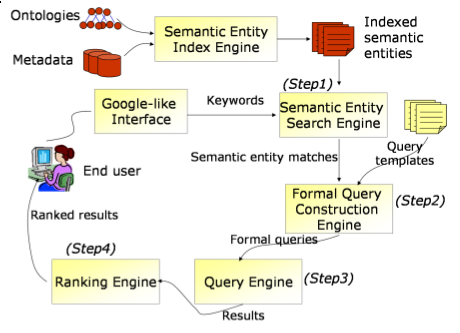
\includegraphics[height = 8cm]{./img/sem_srch.png}\end{center}
SemSearch provides a Google-like query interface allowing users to specify queries without requiring any knowledge about ontologies or specific languages. User queries consist of two or more keywords, whose semantic meaning is taken into account to reformulate the queries themselves according to a formal query language syntax. Keywords are assigned a semantic meaning by matching them against a collection of classes, proper-
ties, and instances in semantic data repositories. Since each keyword can match a class, a property, or an instance, several combinations of semantic matchings of the keywords are considered. For instance, it can be the case that every keyword matches a class, or that the first keyword matches a class, while the second matches a property, and so on. All the combinations of matchings are taken into account in the reformulation process, and each combination leads to a distinguished formal query, obtained from a pre-determined set of query templates. After the reformulation, formal queries are exactly evaluated, and this yields results that are semantically related to all the user keywords.

\subsection{Implementation of Semantic Web}
Up to par, semantic web consits of set of technologies such as semantic graphs, discriptive logic, tagged data, ontologies definnig relationships between entities of web, etc. Some of standards being followed in recent time are RDF, OWL, HTTP, RDFa, etc. OWL and RDF have been growing very popular.


OWL(Web Ontology Language ) is intended to be used when the information contained in documents needs to be processed by applications, as opposed to situations where the content only needs to be presented to humans. OWL can be used to explicitly represent the meaning of terms in vocabularies and the relationships between those terms.

RDF (Resource Description Framework) is a standard model for data interchange on the Web. RDFhas features that facilitate data merging even if the underlying schemas differ, and it specifically supports the evolution of schemas over time without requiring all the data consumers to be
changed. 

Some of the toots used in Semantic Web are Protege, Jena, Sesame, Semantic Media Wiki, etc. A set of popular artifacts implementing Semantic Web are Dbpedia, Cyc and Linkeddata.org.

DBpedia is a project aiming to extract structured content from the information created as part of the Wikipedia project. It allows users to query relationships and properties associated with Wikipedia resources, including links to other related datasets. Cyc is an artificial intelligence project that attempts to assemble a comprehensive ontology and database of everyday common sense knowledge, with the goal of enabling AI applications to perform human-like reasoning. One stated goal is that of providing a completely free and unrestricted semantic vocabulary for use in the Semantic Web.

Linked Data is about using the Web to connect related data that wasn't previously linked, or using the Web to lower the barriers to linking data currently linked using other methods.

\section{Intended Benefits of Semantic Search}
Using the semantic web search end user could exprience new level of satisfaction. Semantic Web as a whole would certainly improve the search, automate topic recognition, better target advertisements, elivate commercial possibilities, save time, save money and so on. There are lots of benifits that everbody on the web could entertain. Some intended benfits that are possible out of this engineering work are :
\begin{description}
\item[Intelligent Search:] Semantic web is representation of the data enveloped inside the doucmuents, multimedias, maps, memos,etc. So using a search to locate those relationally linked data well sturctured in some format, the more meaningful search results could be feed to the end users.
\item[Enhanced Result:] With Semantic Web the web could be programmed to serve more precise information with an ability to manipulate the actual data using some natuaral language processing algorithms or graphs or machine learnings technologies and finally serve the results in multiple dimensions like charts,graphs,pictures,audios,videos or any non verbal apporach rather than a single hyperlink to a page containg the information all in simple human cognitive forms.\begin{quote}\textit{For example:  When somebody search for a piece of information on the web thorugh the interface like sound recording mic/picture, he or she could have some intention to grab some practical and informative results out of it. Meanwhile if the semantic search somehow results some non verbal resutlts like pictures or videos or media associated with it, it would mimimise the gap of the digital divide between the novice user of the web and the data out there on the web. For instance, a farmer growing his/her crop at the field enable enough to use a mobile device could know about what disease his crops are infected with using this search extension. Thats an enhancement, what semantic search is envisoned for.}\end{quote}

\item[Automated Question Answering:] This can be best explained though Knowledge Graph. The Knowledge Graph enables the user to search for things, people or places that Google knows about - landmarks, celebrities, cities, sports teams, buildings, geographical features, movies, celestial objects, works of art and more and instantly get information that’s relevant to the query.

\item[Facilitate controlled vocabulary development:] Web-based solution for simplified development and management of interconnected controlled vocabularies can also facilitated. It would support business stakeholders who need to collaborate on defining and linking enterprise vocabularies, taxonomies, thesauri and ontologies used for information integration, customization and search.
\end{description}

\section{Implementation Problems and Future Possibilites }
A number of semantic search tools have been recently developed. Present semantic search tools are enhancing the performance of traditional search technologies, they are however not suitable for naive users, i.e. ordinary end users who are not necessarily familiar with domain specific semantic data, ontologies, or SQL-like query languages. The semantic search engines should be implemented in such way that it could address these issues:
\begin{itemize}
\item the search engines should tackle the problem of knowledge overhead by supporting a Google like query interface such that the proposed query interface provides a simple but powerful way of specifying queries and also help avoid the undesired typing mistakes.
\item it should address the problem of existing semantic-based keyword search engines by supporting complex queries. It should provide comprehensive means to make sense of user queries and to translate them into formal queries, thus being able to produce precise results that on the one hand satisfy user queries and on the other hand are self-explanatory and understandable by end users.For example support for two or more search phrases seperated by space or some characters: \textit{poverty: Nepal NorthAmerica SouthKorea } 
\item it should be properly desinged and tested so that it serves promising results that is so quick,clean and clear.
\end{itemize}


We have given a brief overview of approaches to semantic search on the Web, which is currently one of the hottest research topics in both the Semantic Web and the Web search community. With the integration of semantic value to the exisiting web, the reasoning capabilities envisioned in Semantic Web technologies are coming to Web search and the Web.Although many approaches and systems to semantic search on the Web already exist, the research in this area is still at the very beginning, and many open research problems still persist. Some of the most pressing research issues\cite{bettina} are maybe:
\begin{enumerate}
\item how to automatically translate natural language queries into formal ontological queries,
\item how to normalise the data to be secure or, alternatively how to mainatin appropirate privacy?
\item how to manage e-commerce complexity, the marketers could have bad practise about advantage over the individuals data.
\item how to automatically add semantic annotations to Web content, or alternatively how to automatically extract knowledge from Web content. 
\item how to consider contextual information to adapt the search results to the needs of the users.
\item how to create and maintain the underlying ontologies. 

  and some of them could be answered as:
  \begin{itemize}
  \item manually by experts, e.g., in a Wikipedia like manner, where different communities may define their own ontologies.
  \item automatically, e.g., by extraction from the Web, eventually coming along with existing pieces of ontological knowledge and annotations (e.g., from existing ontologies or ontology fragments, and/or from existing annotations of Web pages in microformats or RDFa), or
  \item semi-automatically by a combination of both above. 
  \end{itemize}
\end{enumerate}

\section{Conclusion}
As a summary it could be stated that with Semantic Web and Semantic Web Search intgration with web 2.0, the data on the web would be in more managable form i.e  data would be more organised, easy to  retrive in menaningful manners. Even with its primitive exploration, Web is getting smarter, more people are using it, large sets of data are being classified to look patterns, people are using predective modeling, huge comercial usage is eleviating and so on. With this semanitc empowerment of the web, there is a clean sturcturing of the data and user looking behind it.Als these mechanical sevant(electronic devices) are being more useable to our day to day activites. But with this semantic evolution of web there comes some very serious implications like privacy implications, and other issues such as missue of the data for commercial benefits or other advertishments.

Up to now, the sementic web search is at its developinng stage. Performing Web search in the form of returning simple answers to simple questions in natural language is still science fiction. However, with the current activities towards semantic search on the Web, we are moving one step closer to making such desired enviroment.

\begin{thebibliography}{9}
\bibitem{semsrch} Y. Lei, V. S. Uren, and E. Motta. \href{http://citeseerx.ist.psu.edu/viewdoc/download?doi=10.1.1.98.3235\&rep=rep1\&type=pdf}{
    \textit{ SemSearch: A search engine for the Semantic Web.}} In Proc. EKAW-2006, LNCS 4248, pp.238--245. Springer, 2006.

\bibitem{tim} Interview with Sir Tim Berns Lee,by Stev Lohr, The Newyork Times \href{http://blip.tv/beettv/tim-berners-lee-looks-back-the-in-web-addresses-was-unnecessary-2727797} {\textit{
Tim Berners-Lee Looks Back: the "//" in Web Addresses Was Unnecessary}}
\bibitem{bettina} Bettina Fazzinga and Thomas Lukasiewicz. \textit{Semantic search on the Web}.IOS Press,2010.
\bibitem{google} Goole. \url{www.google.com/insidesearch}.
\bibitem{Linked}  Linked Data. \url{http://linkeddata.org/}.
\bibitem {Semanticweb}Semanticweb. \url{http://semanticweb.org/wiki/Cyc}.
\bibitem {Wikipedia}Wikipedia. \url{ en.wikipedia.org/wiki/Semantic_Web}.
\bibitem{Sandro} Sandro Hawke. \href{http://www.w3.org/2002/03/semweb/}{How the Semantic Web Works}. Overview.html,v 1.15 2002/04/22 19:11:29 sandro Exp.

\end{thebibliography}
\end{document}

